\def\difficulty{1}
\sujet{Segmentation of follicles}\index{Segmentation}\index{Mathematical Morphology}

\vspace*{-15pt}

\begin{note}This practical work aims to investigate image segmentation with a direct application to o\-va\-rian follicles. The overall objective is to extract and quantify the granulosa cells and the vascularization of each follicle included in an ewe's ovary.
\end{note}

\vspace*{-5pt}

\noindent The image to be processed is a 2D histological image of an ewe's ovary acquired by optical microscopy in Fig.\ref{fig:follicle:enonce:parts}. The presented image contains one entire follicle (the white region and its neighborhood) and a part of a second one (right-upper corner). The follicle is composed of different parts shown in: antrum, granulosa cells and vascularization. The theca is the ring region around the antrum where the follicle is vascularized.

\vspace*{-10pt}

\begin{figure}[H]
\centering\caption{Different parts of the follicles, to be segmented.}%
\subfloat[Original image with one entire follicle (white region and its neigborhood).]{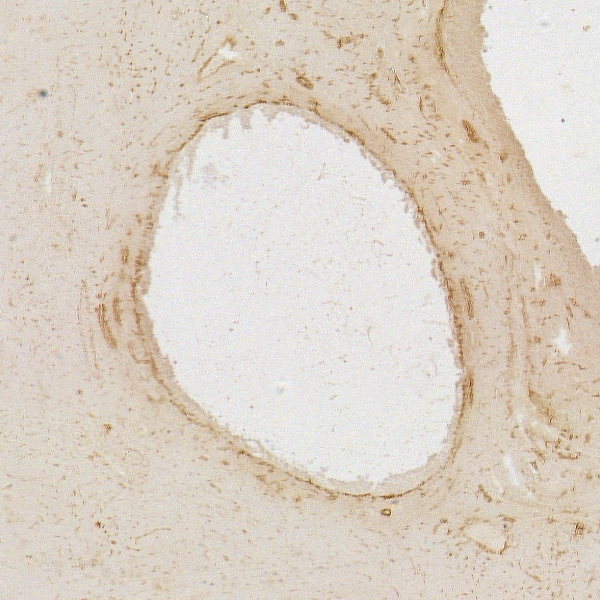
\includegraphics[width=.28\linewidth]{follicule.jpg}}
\hfill
\subfloat[Antrum (dark gray), granu\-lo\-sa cells (light gray) and vas\-cu\-la\-ri\-za\-tion (whi\-te) of the fol\-li\-cle.]{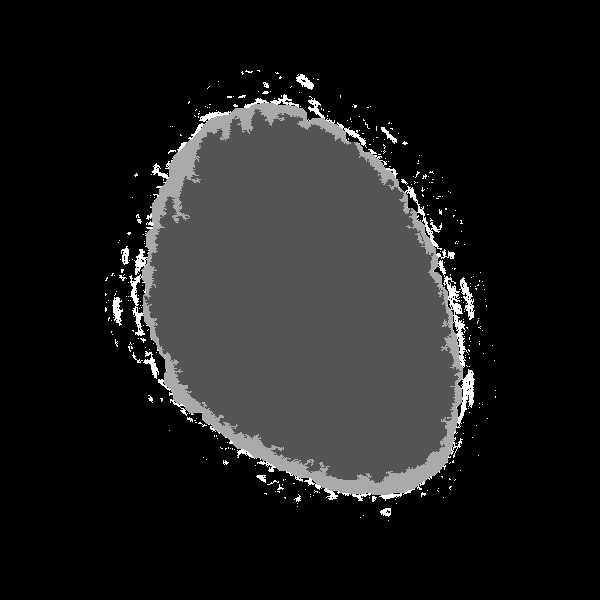
\includegraphics[width=.28\linewidth]{all.png}}
\hfill
\subfloat[Theca.]{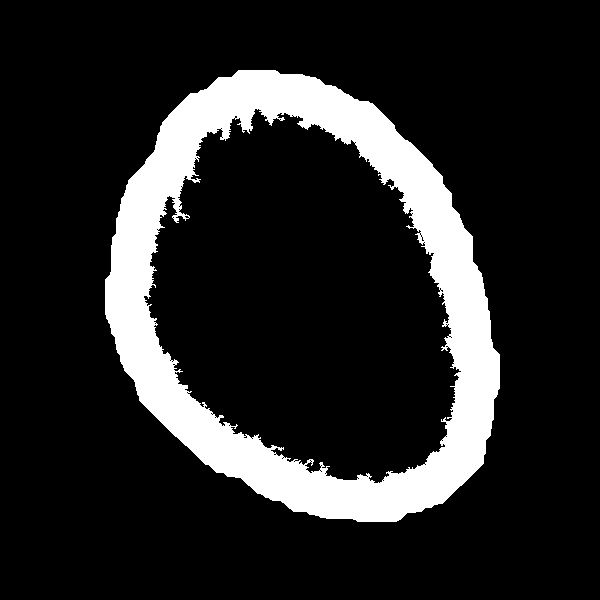
\includegraphics[width=.28\linewidth]{theca.png}}%
\vspace*{-10pt}%
\label{fig:follicle:enonce:parts}%
\end{figure}

\vspace*{-15pt}

\section{Vascularization}
\vspace*{-10pt}
\begin{qbox}
\begin{itemize}
	\item Load and visualize the image.
	\item Extract the antrum of the follicle.
	\item Extract the vascularization (inside a ring around the antrum).
\end{itemize}
\end{qbox}

\vspace*{-10pt}
\section{Granulosa cells}
\vspace*{-10pt}
\begin{qbox}
Which kind of processing could be suitable for extracting the granulosa cells?
\end{qbox}

\vspace*{-10pt}
\section{Quantification}
\vspace*{-10pt}
\begin{qbox}
Provide some geometrical measurements of the different entities of the follicle (antrum, vascularization, granulosa cells).
\end{qbox}
